\documentclass[11pt,aspectratio=169]{beamer}

% Use a clean theme that works well with TikZ
\usetheme{Dresden}
\usecolortheme{crane}

% Use serif fonts for academic look
\usefonttheme{serif}
\usefonttheme{professionalfonts}

% Font packages
\usepackage[T1]{fontenc}
\usepackage{libertine}  % Beautiful serif font
\usepackage[libertine]{newtxmath}  % Matching math font

% Essential TikZ libraries
\usepackage{tikz}
\usetikzlibrary{
    arrows.meta,
    backgrounds,
    calc,
    decorations.pathreplacing,
    decorations.pathmorphing,
    decorations.text,
    fadings,
    fit,
    graphs,
    matrix,
    mindmap,
    patterns,
    positioning,
    shadows,
    shapes.geometric,
    shapes.symbols,
    trees,
    3d,
    automata
}

% PGFPlots for data visualization
\usepackage{pgfplots}
\pgfplotsset{compat=1.18}
\usepgfplotslibrary{statistics}
\usepgfplotslibrary{colorbrewer}

% Colors optimized for TikZ
\definecolor{tikzred}{RGB}{255,58,71}
\definecolor{tikzblue}{RGB}{0,103,184}
\definecolor{tikzgreen}{RGB}{0,146,69}
\definecolor{tikzorange}{RGB}{255,140,0}
\definecolor{tikzpurple}{RGB}{103,78,167}
\definecolor{tikzgray}{RGB}{100,100,100}
\definecolor{lightgray}{RGB}{240,240,240}

% Custom TikZ styles
\tikzset{
    % Box styles
    concept box/.style={
        draw=tikzblue,
        fill=tikzblue!10,
        thick,
        rectangle,
        rounded corners,
        minimum height=1cm,
        minimum width=2.5cm,
        align=center
    },
    data box/.style={
        draw=tikzgreen,
        fill=tikzgreen!10,
        thick,
        rectangle,
        minimum height=0.8cm,
        align=center
    },
    process box/.style={
        draw=tikzorange,
        fill=tikzorange!10,
        thick,
        ellipse,
        minimum height=0.8cm,
        align=center
    },
    % Arrow styles
    flow arrow/.style={
        ->,
        thick,
        >=Stealth,
        tikzblue
    },
    data flow/.style={
        ->,
        thick,
        >=Latex,
        tikzgreen,
        dashed
    },
    % Graph node styles
    main node/.style={
        circle,
        draw=tikzblue,
        fill=tikzblue!20,
        thick,
        minimum size=10mm,
        font=\sffamily\Large
    },
    small node/.style={
        circle,
        draw=tikzpurple,
        fill=tikzpurple!20,
        thick,
        minimum size=6mm
    }
}

% Other packages
\usepackage{amsmath,amssymb,amsthm}
\usepackage{booktabs}
\usepackage{animate}  % For animations with TikZ

% Customize theme colors
\setbeamercolor{structure}{fg=tikzblue}
\setbeamercolor{frametitle}{bg=tikzblue!10}

% Remove navigation
\setbeamertemplate{navigation symbols}{}
\setbeamertemplate{footline}[frame number]

% Title
\title{Advanced Visualization with TikZ}
\subtitle{Interactive Graphics in Academic Presentations}
\author{Dr. Research Scientist}
\institute{Department of Computer Science\\Research University}
\date{\today}

\begin{document}

% Title slide with TikZ decoration
\begingroup
\setbeamertemplate{headline}{} % Remove headline for title slide
\setbeamertemplate{footline}{} % Remove footline for title slide
\setbeamertemplate{navigation symbols}{} % Remove navigation symbols
\setbeamertemplate{background canvas}{
    \begin{tikzpicture}[remember picture,overlay]
        % Plain white background
        \fill[white] (current page.south west) rectangle (current page.north east);
    \end{tikzpicture}
}
\begin{frame}[plain,noframenumbering]
    \vspace{1cm}
    \begin{center}
        {\Huge \textbf{\textcolor{tikzblue}{\inserttitle}}}\\[1em]
        {\Large \textcolor{tikzpurple}{\insertsubtitle}}\\[2em]
        {\large \textcolor{black}{\insertauthor}}\\[0.5em]
        {\textcolor{tikzgray}{\insertinstitute}}\\[1em]
        {\textcolor{tikzgray}{\insertdate}}
    \end{center}
\end{frame}
\endgroup

% Table of Contents
\begin{frame}{Outline}
    \tableofcontents
\end{frame}

% Section 1: Graph Theory Visualizations
\section{Graph Theory with TikZ}

\begin{frame}{Network Topology}
    \begin{center}
    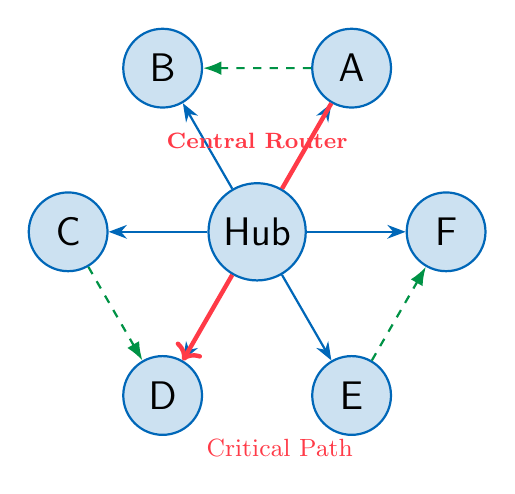
\begin{tikzpicture}[scale=0.8]
        % Define nodes
        \node[main node] (center) at (0,0) {Hub};
        \foreach \i/\label in {1/A,2/B,3/C,4/D,5/E,6/F} {
            \node[main node] (node\i) at ({60*\i}:3) {\label};
        }

        % Draw edges
        \foreach \i in {1,...,6} {
            \draw[flow arrow] (center) -- (node\i);
        }

        % Add some inter-node connections
        \draw[data flow] (node1) -- (node2);
        \draw[data flow] (node3) -- (node4);
        \draw[data flow] (node5) -- (node6);

        % Annotations
        \node[above=0.3cm of center, tikzred, font=\footnotesize\bfseries] {Central Router};

        % Highlight path
        \draw[tikzred, ultra thick, ->] (node1) -- (center) -- (node4);
        \node[tikzred, below right=0.1cm of node4] {\small Critical Path};
    \end{tikzpicture}
    \end{center}

    \begin{block}{Graph Properties}
        \begin{itemize}
            \item Star topology with $n = 6$ leaf nodes
            \item Diameter: 2
            \item Average path length: 1.67
        \end{itemize}
    \end{block}
\end{frame}

\begin{frame}{Binary Tree Structure}
    \begin{columns}
        \begin{column}{0.5\textwidth}
            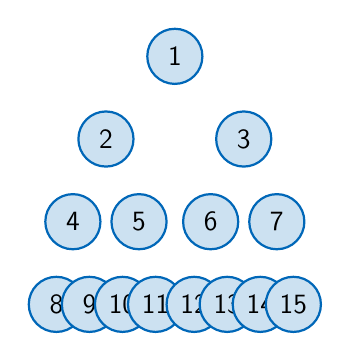
\begin{tikzpicture}[
                scale=0.7,
                level 1/.style={sibling distance=2.5cm},
                level 2/.style={sibling distance=1.2cm},
                level 3/.style={sibling distance=0.6cm},
                every node/.style={main node, scale=0.7},
                edge from parent/.style={flow arrow}
            ]
            \node {1}
                child {node {2}
                    child {node {4}
                        child {node {8}}
                        child {node {9}}
                    }
                    child {node {5}
                        child {node {10}}
                        child {node {11}}
                    }
                }
                child {node {3}
                    child {node {6}
                        child {node {12}}
                        child {node {13}}
                    }
                    child {node {7}
                        child {node {14}}
                        child {node {15}}
                    }
                };
            \end{tikzpicture}
        \end{column}

        \begin{column}{0.5\textwidth}
            \textbf{Tree Properties:}
            \begin{itemize}
                \item Height: 3
                \item Nodes: 15
                \item Complete binary tree
            \end{itemize}

            \vspace{0.5em}

            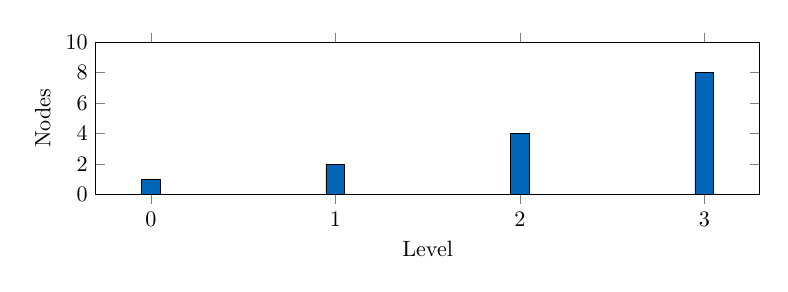
\begin{tikzpicture}[scale=0.8]
                \begin{axis}[
                    ybar,
                    bar width=0.3cm,
                    xlabel={Level},
                    ylabel={Nodes},
                    ymin=0, ymax=10,
                    xtick={0,1,2,3},
                    width=\textwidth,
                    height=4cm
                ]
                \addplot[fill=tikzblue] coordinates {(0,1) (1,2) (2,4) (3,8)};
                \end{axis}
            \end{tikzpicture}
        \end{column}
    \end{columns}
\end{frame}

% Section 2: Flowcharts and Algorithms
\section{Algorithm Visualization}

\begin{frame}{Algorithm Flowchart}
    \begin{center}
    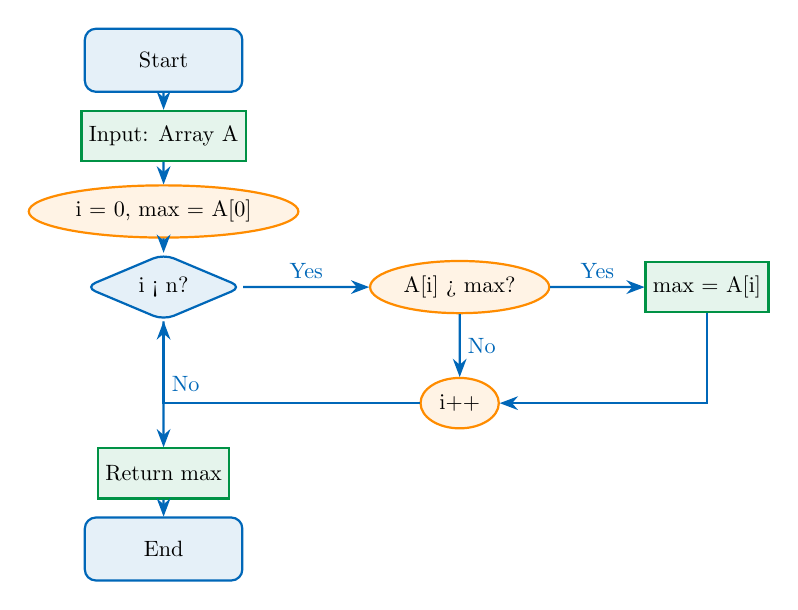
\begin{tikzpicture}[node distance=1.2cm, scale=0.8, transform shape]
        % Nodes
        \node[concept box] (start) {Start};
        \node[data box, below of=start] (input) {Input: Array A};
        \node[process box, below of=input] (init) {i = 0, max = A[0]};
        \node[concept box, below of=init, diamond, aspect=2] (decision) {i < n?};
        \node[process box, right=2cm of decision] (compare) {A[i] > max?};
        \node[data box, right=1.5cm of compare] (update) {max = A[i]};
        \node[process box, below=1cm of compare] (increment) {i++};
        \node[data box, below=2cm of decision] (output) {Return max};
        \node[concept box, below of=output] (end) {End};

        % Edges
        \draw[flow arrow] (start) -- (input);
        \draw[flow arrow] (input) -- (init);
        \draw[flow arrow] (init) -- (decision);
        \draw[flow arrow] (decision) -- node[above] {Yes} (compare);
        \draw[flow arrow] (compare) -- node[above] {Yes} (update);
        \draw[flow arrow] (compare) -- node[right] {No} (increment);
        \draw[flow arrow] (update) |- (increment);
        \draw[flow arrow] (increment) -| (decision);
        \draw[flow arrow] (decision) -- node[right] {No} (output);
        \draw[flow arrow] (output) -- (end);
    \end{tikzpicture}
    \end{center}
\end{frame}

\begin{frame}{Sorting Algorithm Visualization}
    \begin{center}
    \textbf{Bubble Sort Steps}

    \vspace{0.3em}

    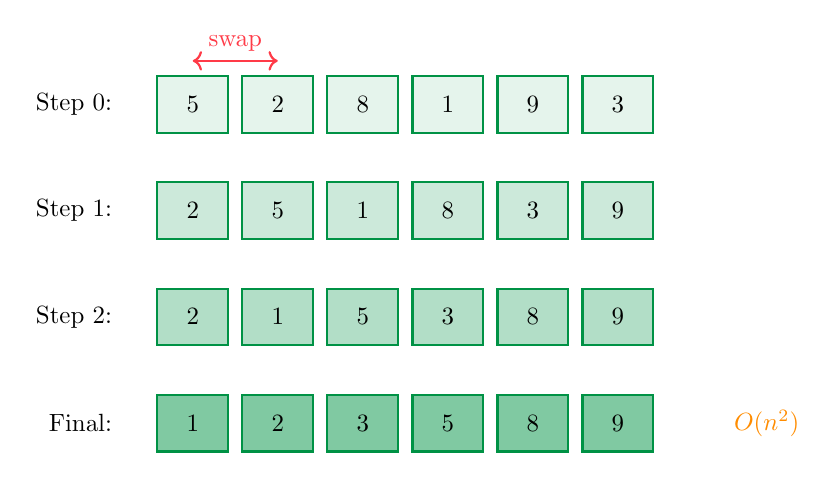
\begin{tikzpicture}[scale=0.9, transform shape]
        % Initial array
        \foreach \i/\val in {0/5,1/2,2/8,3/1,4/9,5/3} {
            \node[data box, minimum width=1cm] at (\i*1.2,0) (a\i) {\val};
        }
        \node[left=0.5cm of a0] {Step 0:};

        % Step 1
        \foreach \i/\val in {0/2,1/5,2/1,3/8,4/3,5/9} {
            \node[data box, minimum width=1cm, fill=tikzgreen!20] at (\i*1.2,-1.5) (b\i) {\val};
        }
        \node[left=0.5cm of b0] {Step 1:};
        \draw[tikzred, thick, <->] ([yshift=0.2cm]a0.north) -- node[above] {swap} ([yshift=0.2cm]a1.north);

        % Step 2
        \foreach \i/\val in {0/2,1/1,2/5,3/3,4/8,5/9} {
            \node[data box, minimum width=1cm, fill=tikzgreen!30] at (\i*1.2,-3) (c\i) {\val};
        }
        \node[left=0.5cm of c0] {Step 2:};

        % Final
        \foreach \i/\val in {0/1,1/2,2/3,3/5,4/8,5/9} {
            \node[data box, minimum width=1cm, fill=tikzgreen!50] at (\i*1.2,-4.5) (d\i) {\val};
        }
        \node[left=0.5cm of d0] {Final:};

        % Complexity annotation
        \node[right=1cm of d5, tikzorange] {$O(n^2)$};
    \end{tikzpicture}
    \end{center}
\end{frame}

% Section 3: Data Visualization
\section{Data Visualization}

\begin{frame}{3D Visualization}
    \begin{columns}
        \begin{column}{0.5\textwidth}
            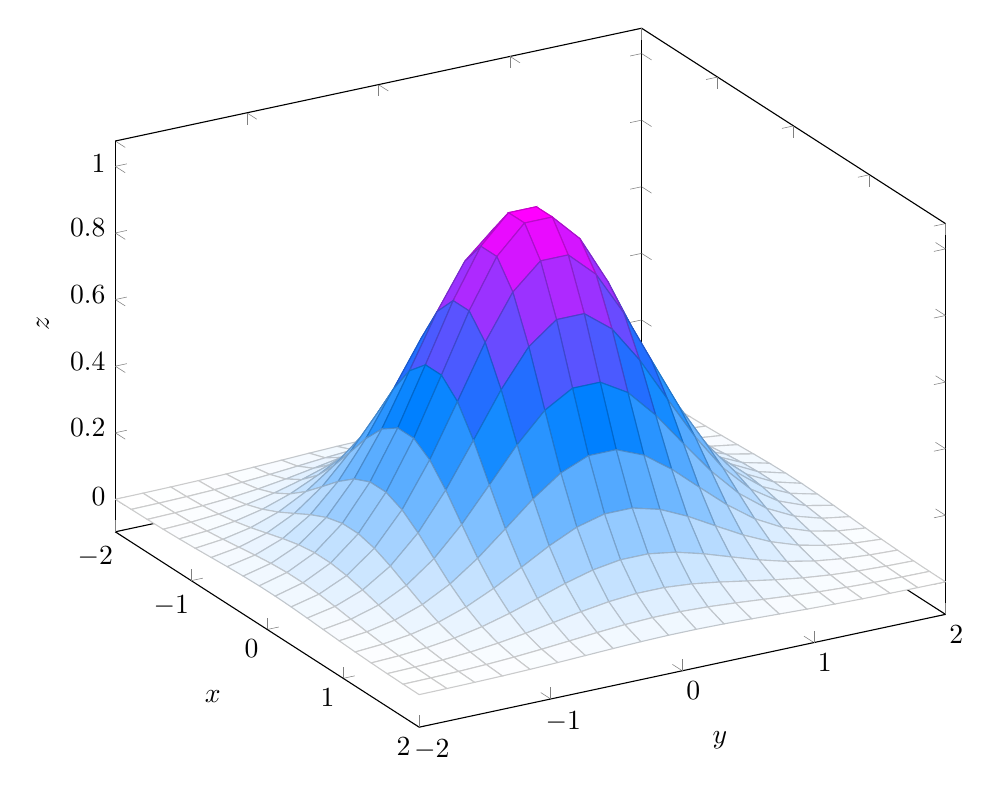
\begin{tikzpicture}
                \begin{axis}[
                    view={60}{30},
                    width=\textwidth,
                    xlabel=$x$,
                    ylabel=$y$,
                    zlabel=$z$,
                    colormap/cool,
                ]
                \addplot3[
                    surf,
                    domain=-2:2,
                    domain y=-2:2,
                    samples=20,
                ] {exp(-x^2-y^2)};
                \end{axis}
            \end{tikzpicture}

            \centering
            Gaussian Distribution
        \end{column}

        \begin{column}{0.5\textwidth}
            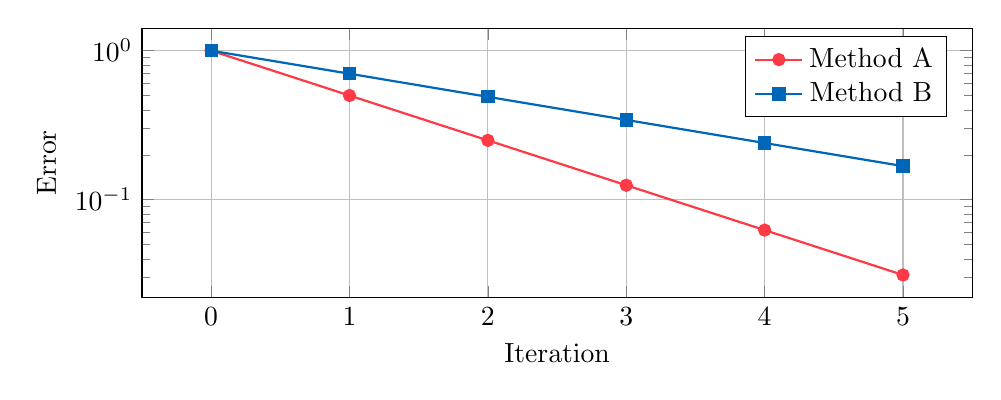
\begin{tikzpicture}
                \begin{axis}[
                    width=\textwidth,
                    height=5cm,
                    xlabel={Iteration},
                    ylabel={Error},
                    ymode=log,
                    legend pos=north east,
                    grid=major,
                ]
                \addplot[tikzred, thick, mark=*] coordinates {
                    (0,1) (1,0.5) (2,0.25) (3,0.125) (4,0.0625) (5,0.03125)
                };
                \addplot[tikzblue, thick, mark=square*] coordinates {
                    (0,1) (1,0.7) (2,0.49) (3,0.343) (4,0.240) (5,0.168)
                };
                \legend{Method A, Method B}
                \end{axis}
            \end{tikzpicture}

            \centering
            Convergence Analysis
        \end{column}
    \end{columns}
\end{frame}

\begin{frame}{Statistical Charts}
    \begin{columns}
        \begin{column}{0.5\textwidth}
            \centering
            \textbf{Distribution Analysis}

            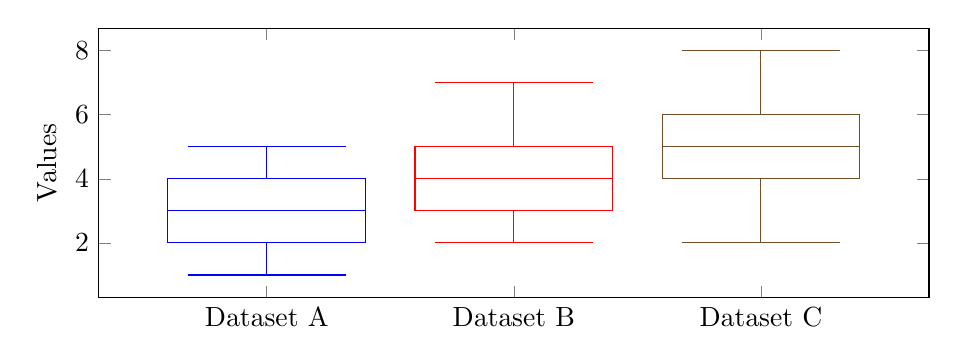
\begin{tikzpicture}
                \begin{axis}[
                    width=\textwidth,
                    height=5cm,
                    boxplot/draw direction=y,
                    ylabel={Values},
                    xtick={1,2,3},
                    xticklabels={Dataset A, Dataset B, Dataset C},
                ]
                \addplot+[boxplot prepared={
                    median=3,
                    upper quartile=4,
                    lower quartile=2,
                    upper whisker=5,
                    lower whisker=1
                }] coordinates {};
                \addplot+[boxplot prepared={
                    median=4,
                    upper quartile=5,
                    lower quartile=3,
                    upper whisker=7,
                    lower whisker=2
                }] coordinates {};
                \addplot+[boxplot prepared={
                    median=5,
                    upper quartile=6,
                    lower quartile=4,
                    upper whisker=8,
                    lower whisker=2
                }] coordinates {};
                \end{axis}
            \end{tikzpicture}
        \end{column}

        \begin{column}{0.5\textwidth}
            \centering
            \textbf{Category Comparison}

            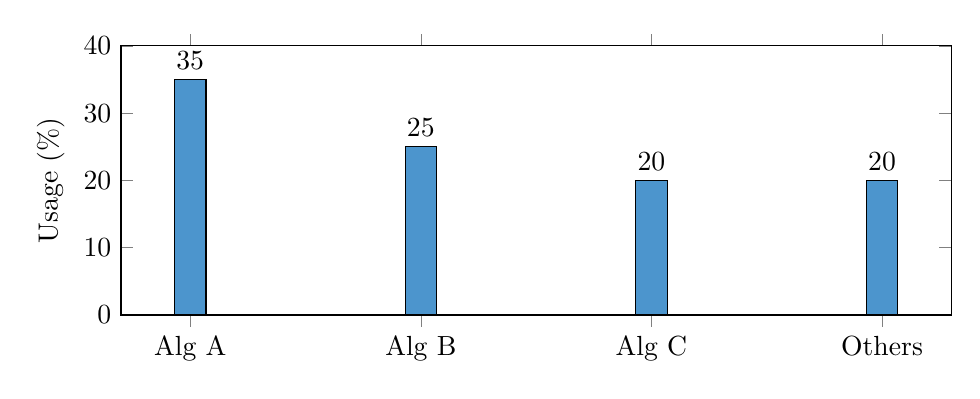
\begin{tikzpicture}
                \begin{axis}[
                    ybar,
                    bar width=0.4cm,
                    symbolic x coords={Alg A, Alg B, Alg C, Others},
                    xtick=data,
                    ylabel={Usage (\%)},
                    ymin=0, ymax=40,
                    nodes near coords,
                    width=\textwidth,
                    height=5cm
                ]
                \addplot[fill=tikzblue!70] coordinates {
                    (Alg A, 35) (Alg B, 25) (Alg C, 20) (Others, 20)
                };
                \end{axis}
            \end{tikzpicture}
        \end{column}
    \end{columns}
\end{frame}

% Section 4: Mind Maps
\section{Conceptual Diagrams}

\begin{frame}{Mind Map}
    \begin{center}
    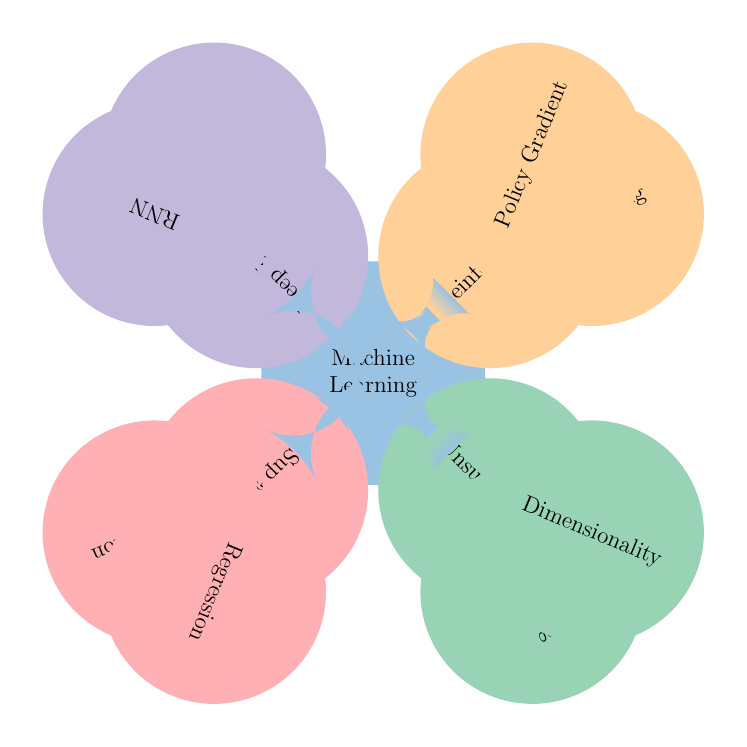
\begin{tikzpicture}[mindmap, grow cyclic, every node/.style=concept, concept color=tikzblue!40,
        scale=0.7, transform shape,
        level 1/.style={level distance=3cm,sibling angle=90},
        level 2/.style={level distance=2cm,sibling angle=45}]

        \node[concept] {Machine\\Learning}
            child[concept color=tikzred!40] { node {Supervised}
                child { node {Classification} }
                child { node {Regression} }
            }
            child[concept color=tikzgreen!40] { node {Unsupervised}
                child { node {Clustering} }
                child { node {Dimensionality} }
            }
            child[concept color=tikzorange!40] { node {Reinforcement}
                child { node {Q-Learning} }
                child { node {Policy Gradient} }
            }
            child[concept color=tikzpurple!40] { node {Deep Learning}
                child { node {CNN} }
                child { node {RNN} }
            };
    \end{tikzpicture}
    \end{center}
\end{frame}

\begin{frame}{System Architecture}
    \begin{center}
    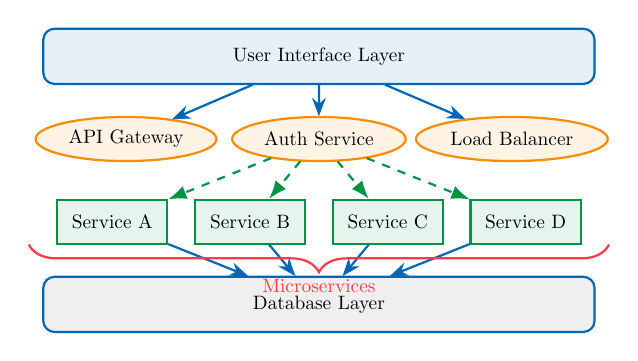
\begin{tikzpicture}[scale=0.7, transform shape]
        % Define layers
        \begin{scope}[yshift=3cm]
            \node[concept box, minimum width=10cm] (ui) {User Interface Layer};
        \end{scope}

        \begin{scope}[yshift=1.5cm]
            \foreach \i/\name in {0/API Gateway,1/Auth Service,2/Load Balancer} {
                \node[process box, minimum width=2.8cm] at (\i*3.5-3.5,0) (service\i) {\name};
            }
        \end{scope}

        \begin{scope}
            \foreach \i/\name in {0/Service A,1/Service B,2/Service C,3/Service D} {
                \node[data box, minimum width=2cm] at (\i*2.5-3.75,0) (micro\i) {\name};
            }
        \end{scope}

        \begin{scope}[yshift=-1.5cm]
            \node[concept box, minimum width=10cm, fill=tikzgray!10] (db) {Database Layer};
        \end{scope}

        % Connections
        \draw[flow arrow] (ui) -- (service0);
        \draw[flow arrow] (ui) -- (service1);
        \draw[flow arrow] (ui) -- (service2);

        \foreach \i in {0,1,2,3} {
            \draw[data flow] (service1) -- (micro\i);
        }

        \foreach \i in {0,1,2,3} {
            \draw[flow arrow] (micro\i) -- (db);
        }

        % Annotations
        \draw[decorate, decoration={brace,amplitude=10pt,mirror}, tikzred, thick]
            ([xshift=-0.5cm]micro0.south west) -- ([xshift=0.5cm]micro3.south east)
            node[midway, below=0.5cm, tikzred] {Microservices};
    \end{tikzpicture}
    \end{center}
\end{frame}

% Section 5: Animated Diagrams
\section{Advanced Features}

\begin{frame}{State Machine}
    \begin{center}
    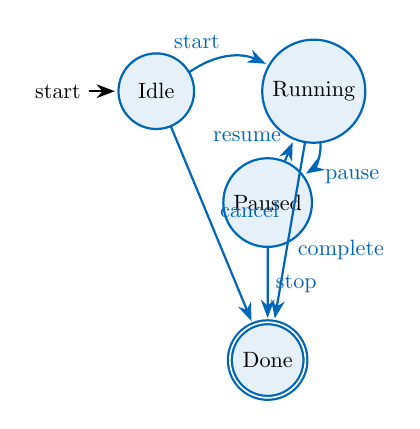
\begin{tikzpicture}[
        scale=0.8, transform shape,
        ->,>=Stealth,
        shorten >=1pt,
        auto,
        node distance=2.5cm,
        thick,
        every state/.style={
            draw=tikzblue,
            fill=tikzblue!10,
            thick,
            minimum size=1.2cm
        }
    ]

        \node[state, initial] (idle) {Idle};
        \node[state] (running) [right of=idle] {Running};
        \node[state] (paused) [below right of=idle] {Paused};
        \node[state, accepting] (done) [below of=paused] {Done};

        \path[flow arrow]
            (idle) edge[bend left] node {start} (running)
            (running) edge[bend left] node {pause} (paused)
            (paused) edge node {resume} (running)
            (running) edge node {complete} (done)
            (paused) edge node {stop} (done)
            (idle) edge node {cancel} (done);
    \end{tikzpicture}
    \end{center}

    \begin{block}{State Transitions}
        Total states: 4, Total transitions: 6, Terminal state: Done
    \end{block}
\end{frame}

\begin{frame}{Timeline Visualization}
    \begin{center}
    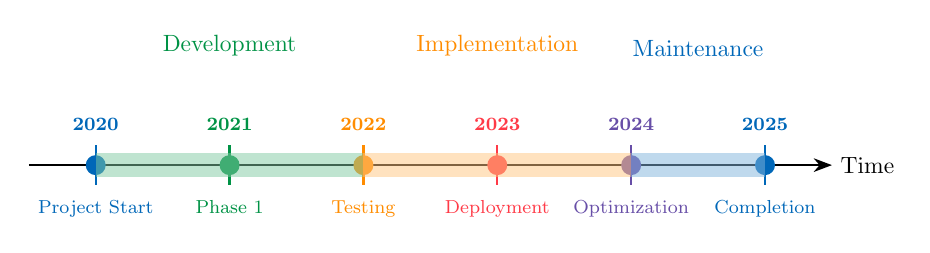
\begin{tikzpicture}[scale=0.85, transform shape]
        % Timeline
        \draw[thick, ->, >=Stealth] (0,0) -- (12,0) node[right] {Time};

        % Events - Manual placement to avoid foreach issues
        \draw[thick, tikzblue] (1,0) -- (1,0.3);
        \draw[thick, tikzblue] (1,0) -- (1,-0.3);
        \node[above=0.4cm, tikzblue, font=\footnotesize\bfseries] at (1,0) {2020};
        \node[below=0.4cm, tikzblue, font=\footnotesize, align=center] at (1,0) {Project Start};
        \node[circle, fill=tikzblue, inner sep=3pt] at (1,0) {};

        \draw[thick, tikzgreen] (3,0) -- (3,0.3);
        \draw[thick, tikzgreen] (3,0) -- (3,-0.3);
        \node[above=0.4cm, tikzgreen, font=\footnotesize\bfseries] at (3,0) {2021};
        \node[below=0.4cm, tikzgreen, font=\footnotesize, align=center] at (3,0) {Phase 1};
        \node[circle, fill=tikzgreen, inner sep=3pt] at (3,0) {};

        \draw[thick, tikzorange] (5,0) -- (5,0.3);
        \draw[thick, tikzorange] (5,0) -- (5,-0.3);
        \node[above=0.4cm, tikzorange, font=\footnotesize\bfseries] at (5,0) {2022};
        \node[below=0.4cm, tikzorange, font=\footnotesize, align=center] at (5,0) {Testing};
        \node[circle, fill=tikzorange, inner sep=3pt] at (5,0) {};

        \draw[thick, tikzred] (7,0) -- (7,0.3);
        \draw[thick, tikzred] (7,0) -- (7,-0.3);
        \node[above=0.4cm, tikzred, font=\footnotesize\bfseries] at (7,0) {2023};
        \node[below=0.4cm, tikzred, font=\footnotesize, align=center] at (7,0) {Deployment};
        \node[circle, fill=tikzred, inner sep=3pt] at (7,0) {};

        \draw[thick, tikzpurple] (9,0) -- (9,0.3);
        \draw[thick, tikzpurple] (9,0) -- (9,-0.3);
        \node[above=0.4cm, tikzpurple, font=\footnotesize\bfseries] at (9,0) {2024};
        \node[below=0.4cm, tikzpurple, font=\footnotesize, align=center] at (9,0) {Optimization};
        \node[circle, fill=tikzpurple, inner sep=3pt] at (9,0) {};

        \draw[thick, tikzblue] (11,0) -- (11,0.3);
        \draw[thick, tikzblue] (11,0) -- (11,-0.3);
        \node[above=0.4cm, tikzblue, font=\footnotesize\bfseries] at (11,0) {2025};
        \node[below=0.4cm, tikzblue, font=\footnotesize, align=center] at (11,0) {Completion};
        \node[circle, fill=tikzblue, inner sep=3pt] at (11,0) {};

        % Phases
        \draw[tikzgreen!50, line width=3mm, opacity=0.5] (1,0) -- (5,0);
        \draw[tikzorange!50, line width=3mm, opacity=0.5] (5,0) -- (9,0);
        \draw[tikzblue!50, line width=3mm, opacity=0.5] (9,0) -- (11,0);

        \node[above=1.5cm, tikzgreen] at (3,0) {Development};
        \node[above=1.5cm, tikzorange] at (7,0) {Implementation};
        \node[above=1.5cm, tikzblue] at (10,0) {Maintenance};
    \end{tikzpicture}
    \end{center}
\end{frame}

% Conclusion
\section{Conclusion}

\begin{frame}{Summary}
    \begin{columns}
        \begin{column}{0.5\textwidth}
            \textbf{TikZ Capabilities Demonstrated:}
            \begin{itemize}
                \item Graph and tree structures
                \item Flowcharts and algorithms
                \item 3D visualizations
                \item Statistical charts
                \item Mind maps
                \item State machines
                \item Timeline graphics
            \end{itemize}
        \end{column}

        \begin{column}{0.5\textwidth}
            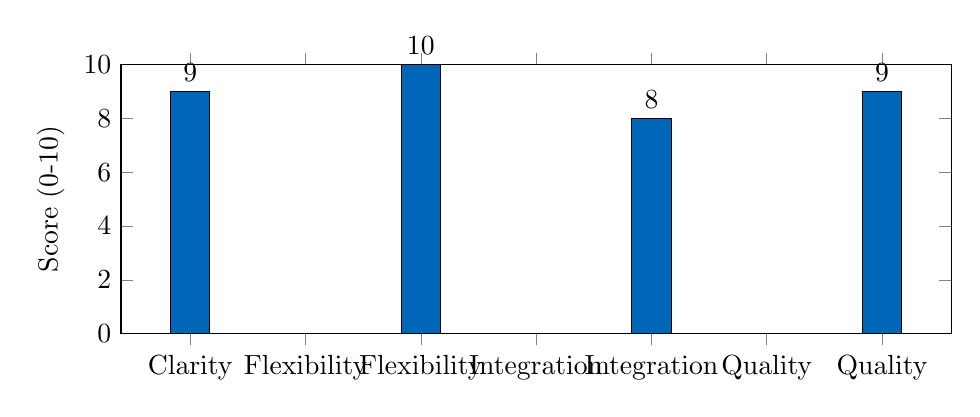
\begin{tikzpicture}
                \begin{axis}[
                    symbolic x coords={Clarity,Flexibility,Integration,Quality},
                    ylabel={Score (0-10)},
                    ybar,
                    bar width=0.5cm,
                    ymin=0,
                    ymax=10,
                    nodes near coords,
                    width=\textwidth,
                    height=5cm
                ]
                \addplot[fill=tikzblue] coordinates {
                    (Clarity,9) (Flexibility,10) (Integration,8) (Quality,9)
                };
                \end{axis}
            \end{tikzpicture}

            \centering
            \textbf{TikZ Advantages}
        \end{column}
    \end{columns}

    \vspace{1em}

    \begin{center}
        \textbf{Thank you for your attention!}
    \end{center}
\end{frame}

\end{document}